\section{RDS: Astronomy and Astrophysics}
\label{sect:rds}

\sectauthor{Markus Demleitner, Univ.~Heidelberg}

\subsection{Existing Federated Infrastructures}

The Virtual Observatory (VO) is an international effort to run and
develop a federated data infrastructure in Astronomy that is held
together by a set of data and protocol standards, continually developed
since the early 2000s.  Consisting of a Registry, some 25000
interoperable services (which still roughly match data collections)
comprising hundreds of millions of datasets (spectra, images, and the
like) and hundreds of billions of table rows, and a set of clients and
libraries consuming these services, it is widely used in the
astronomical community.

One central assumption behind the VO is that users should not normally
interact with data services -- machines should do that on their behalf.
This is to facilitate using many different services at the same time
(``global discovery''; here, a client can easily query hundreds of
services, where no human would fill out hundreds of web forms) or
sequentially (avoiding ``lock-in'' to specific services or resources;
standard services save exploration time).

A \emph{VO service} thus is a network-accessible endpoint defined by 
our \emph{standards}, giving access to one or more data collections.  
To illustrate the VO's approach, here is a hypothetical session:

Suppose a user requests ``images of Barnard's
star in x-rays''.  This is how this proceeds in the VO:

\begin{enumerate}
\item A client asks a searchable registry: Give me resources that
\begin{itemize}
\item serve images,
\item have data in the x-ray part of the spectrum, and
\item have data around $\alpha=269.45$, $\delta=4.693$ (i.e., the
current location of Barnard's star in the sky).
\end{itemize}
\item The Registry responds with metadata for the services 
matching these criteria.
\item The client now goes to each service returned and asks it for
data
\begin{itemize}
\item covering the position $\alpha=269.45$, $\delta=4.693$ and
\item intersecting the spectral range $0.1\cdots 120\,\rm keV$ of
photon energy.
\end{itemize}
\item Each server responds with one set of metadata per matched image. 
The client turns this into some representation for the user.
\item The user picks images based on the metadata (e.g., observation
date, sensitivity\dots).
\item The client retrieves image (or parts of them) and makes them
available for further processing.
\end{enumerate}

\begin{figure}[t]
\hbox to \textwidth{\hfil
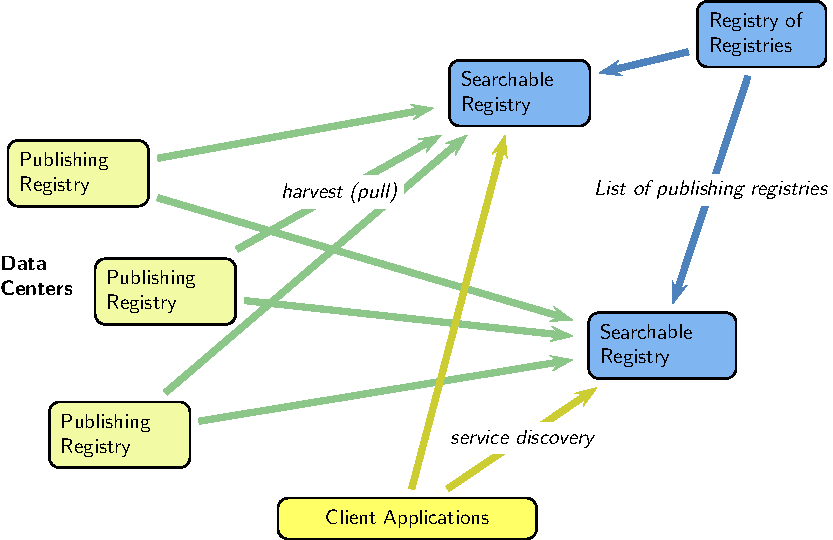
\includegraphics[width=0.8\textwidth]{rds-regexchange.pdf}\hfil}

\caption{The architecture of the VO Registry: Service discovery happens
using \emph{searchable registries}.  While anyone can run one, in
practice there are three major operators (GAVO, ESA, STScI) that clients
can go to as they choose.  These searchable registries get their data by
OAI-PMH harvesting \emph{publishing registries} operated by the data
providers.  They know where to go because all (currently about 45)
publishing registries are listed in the one central infrastructure of
the VO, the \emph{RofR} (Registry of Registries).}

\label{fig:rds-regexchange}
\end{figure}

Here is a brief overview of the standards that have been developed in
the context of the VO effort:

\textbf{Searching for data:} Images (SIAP), spectra (SSAP), objects
(SCS), spectral lines (SLAP), generic datasets (ObsCore).

\textbf{Remote manipulation:} SODA, specifying cutouts, rescaling, etc.,
to avoid pulling data not relevant to the user.

\textbf{Interacting with databases:} Access using TAP, common query
language ADQL.

\textbf{Formats:} Table exchange using VOTable, complex spherical
geometries with MOC, multiscale images with HiPS.

\textbf{Registry:} Registry Interfaces for the architecture, VOResource,
VODataService, TAPRegExt, SimpleDALRegExt for the metadata format,
RegTAP for how to search it.

\textbf{Semantics:} Light semantics of physical quantities (UCD), Unit
syntax, vocabulary maintenance, $\sim 15$ vocabularies.

\textbf{Other:} SAMP for assembling complex environments from simple
building blocks, VOSpace as an object store, VOEvent for disseminating
information in transient phenomena in the sky.

The full list of IVOA standards is available from the IVOA document
repository\footnote{\url{http://ivoa.net/documents}}.  The IVOA also
takes up a large number of third-party standards, in particular many
IETF and W3C standards including HTTP, RDF, and XML, as well as FITS and
OAI-PMH, or the Unified Astronomy Thesaurus maintained by journal
publishers, librarians and learned societies.

A cornerstone of the VO is the Registry; Fig.~\ref{fig:rds-regexchange}
illustrates its architecture, designed both to avoid operation-critical
central components and in the VO spirit of letting, in principle,
anyone offer any sort of service.  The only part in the VO Registry that
is actually a central singleton is the Registry of Registries, and that
can, if necessary, be unavailable for days without noticable impact on
VO users.

\subsection{Technologies Employed}

Central to most of what the VO does are relational databases -- most
projects run Postgres, but many other RDBMSes are in use, too.
This is partly because a relevant part of our science data
(``catalogues'') is relational in nature, partly because our discovery
interfaces for datasets are written in terms of relational
representations.

Some rather basic structures were developed within the discipline; a
good example is MOC and the associated HiPS, techniques for the fast
representation of rather arbitrary regions on spheres and information
linked to such regions (think research-quality Google Earth).

Our Registry's metadata scheme is significantly more elaborate than
DataCite's, in particularly adding metadata on tables and services.
Mapping the VOResource to DataCite is rather straightforward but loses
almost all the metadata that actually makes the VO work.

Really central to the VO are end-user components.  These can roughly be
grouped into Browser-based ones (e.g., ESA sky for general browsing,
WIRR for registry discovery), Applications (which, for deployment
convenience, are mostly written Java; popular examples include TOPCAT
and Aladin), and libraries for VO access (e.g., pyVO and astroquery from
Python, which by now are the most popular programmatic interfaces among
end users, STIL from Java).  In particular the early VO had a tendency
to forget about these client parts, and whenever it did that, things
quickly went awry.

For worked-out use cases for VO operations, see VO Text
Treasures\footnote{\url{https://dc.g-vo.org/VOTT}}.

\subsection{Current Issues}

One major challenge is how to deal with data too large to conveniently
move.  While with the SQL derivative ADQL and the query-transporting
Table Access Protocol TAP we have a highly successful model for how to
bring expressions from relational algebra to the data, similarly clear and
interoperable techniques for array-like data, let alone collections of
arrays (e.g., images, dynamic spectra, complex time series) have yet to
be developed; that these techniques will probably involve
Turing-complete formalisms that are hard to reason about even for
machines exarcerbates the situation.  

Right now, observatories facing the problem of data that is hard to move
tend to offer services based on containers or ipython backends, but of
course these are neither interoperable (in the sense that a, say,
ipython notebook could be easily transferred from one service to
another) nor discoverable, and at least compared with ADQL queries (that
will still work even if they were written 10 years ago) they will break
rather quickly due to evolving dependencies.

On thing we are still struggling with was the early design of
identifying data collections and services, where, say, a collection of
spectra was registered as a service for searching spectra.  This was
initially convenient but became increasingly cumbersome as services
started to publish multiple data collections -- there are several
services in today's VO offering more than a thousand data collections
each behind a single access URL -- and data collections became available
through multiple interfaces -- it is rather common today for datasets
to be published through both a typed interface (SIAP, SSAP) and through
a TAP-published table containing standard metadata for observational data
(obscore).  Rectifying this early misdesign while widely deployed
clients will break on straightforward fixes has proven to be a major
challenge.

What has not really worked in the VO so far is data modelling.  While
data models have been proposed for both concrete data products (e.g.,
Spectra) and physical concepts (e.g., positions, photometry), takeup for
whatever prescriptions were derived from these has been low, and clients
essentially do not consume them.  On the other hand, there is a clear
need for having more complex data structures described interoperably.
There is an effort underway to rectify the situation by a stronger
formalisation of modelling work using an interoperable subset of UML
(``VO-DML'') and standard serialisation of instances.  On the other
hand, given the predominance of relational databases in the VO, direct
modelling in relational terms (e.g., ObsCore, RegTAP, EPN-TAP, Datalink)
has been rather successful.

For Germany, a central problem with respect to the VO is that there is
essentially no institutional footing.  Where France has the CDS, Canada
the CADC, the US at least MAST and IRSA, the UK the WFAU, and Italy
INAF's Trieste data centre, the German contribution to the VO has so far
relied mostly on BMBF and EU project funding, which is both uncertain
and strongly fluctuating.  An institutional basis would make our
contribution significantly more sustainable and credible.


\subsection{Infrastructures to be Federated}

As said above, compute platforms next to immovable data should be made
interoperable and discoverable, but that clearly is a hard problem without
simple solutions.  Perhaps going some smaller steps initially, e.g.,
using techniques like ArraySQL, will help to find paths towards more
general and simultaneously viable solutions.

A constant problem since the early days of the VO has been
authentication.  It has not been particularly pressing so far, as open
data is rather common in astronomy, but with advanced services like
persistent uploads on TAP services and computing platforms,
the lack of interoperable, widely implemented, federated authentication
is becoming a hindrance.  What standards have been written in this field
(SSO, Credential Delegation), are either not sufficiently constraining
to enable implementations against them or are not implemented widely
enough.
